%% img/RecursiveHierarchy.tex
%% Copyright 2019 Andrea Berlingieri
%
% This work may be distributed and/or modified under the
% conditions of the LaTeX Project Public License, either version 1.3
% of this license or (at your option) any later version.
% The latest version of this license is in
%   http://www.latex-project.org/lppl.txt
% and version 1.3 or later is part of all distributions of LaTeX
% version 2005/12/01 or later.
%
% This work has the LPPL maintenance status `maintained'.
%
% The Current Maintainer of this work is Andrea Berlingieri.
%
% This work consists of all files listed in manifest.txt
\documentclass{standalone}

\usepackage{../TikzStyle}
\usepackage{../mystyle}

\begin{document}
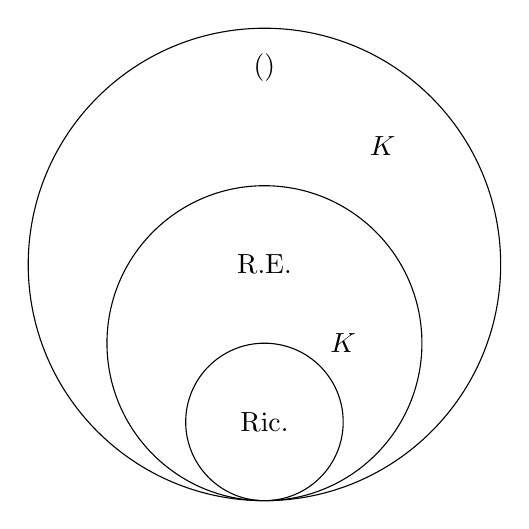
\begin{tikzpicture}
    \draw (0,0) circle [radius=3cm];
    \draw (0,-1) circle [radius=2cm];
    \draw (0,-2) circle [radius=1cm];
    \node at (0,2.5) {$\Parts(\Nat)$};
    \node at (1.5,1.5) {$\comp{K}$};
    \node at (0,0) {R.E.};
    \node at (1,-1) {$K$};
    \node at (0,-2) {Ric.};
\end{tikzpicture}
\end{document}
